\documentclass[11pt]{article}
\usepackage{amsmath, amssymb, mathtools, bm}
\usepackage{physics}
\usepackage{tikz}
\usetikzlibrary{decorations.markings, decorations.pathmorphing, arrows.meta, positioning, calc}
\usepackage{pgfplots}
\pgfplotsset{compat=1.18}
\usepackage[margin=2.3cm]{geometry}
\usepackage{siunitx, booktabs, hyperref}
\usepackage{braket}

\newcommand{\D}{\mathrm{D}}
\newcommand{\de}{\mathrm{d}}
\newcommand{\pd}[2]{\frac{\partial #1}{\partial #2}}
\newcommand{\pdd}[2]{\frac{\partial^{2} #1}{\partial #2^{2}}}
\newcommand{\Lap}{\nabla^{2}}

\title{B4 --- Nuclear and Particle Physics \\ Model Solutions, Trinity 2024}
\author{}
\date{}

\begin{document}
\maketitle

% =========================================================================
\section*{Question 1 --- Nuclear form factors and electron scattering}

\textbf{Problem.} Define $F(q)$ for elastic charged-particle--nucleus scattering; compute it for a uniform sphere; analyse limits and softening of minima; state the relativistic correction; estimate $E_{\min}$ for $R=\SI{3}{fm}$.

\subsection*{(a) The form factor and its evaluation for a uniform sphere}

Born amplitude for a point nucleus is the Rutherford amplitude $f_R(q)$. For an extended charge density $\rho(\vb r)$ with $\int\rho\,\de^{3}r=Ze$:
\begin{equation}
f(\vb q)\;=\;f_R(q)\,F(\vb q),\qquad F(\vb q)\;=\;\frac{1}{Ze}\int\rho(\vb r)\,e^{i\vb q\cdot\vb r/\hbar}\,\de^{3}r.
\label{eq:F-def}
\end{equation}
Differential cross-section: $\de\sigma/\de\Omega=(\de\sigma/\de\Omega)_\text{Ruth}\,|F(q)|^{2}$, with $F(0)=1$.

Spherical symmetry, polar axis along $\vb q$, angular integral $\int_{-1}^{1}e^{iqr\cos\theta/\hbar}\de\cos\theta=2\sin(qr/\hbar)/(qr/\hbar)$:
\begin{equation}
F(q)\;=\;\frac{4\pi}{Ze}\int_{0}^{\infty}\rho(r)\,\frac{\sin(qr/\hbar)}{qr/\hbar}\,r^{2}\,\de r.
\label{eq:F-spherical}
\end{equation}
Set $\hbar=1$ henceforth.

Uniform sphere: $\rho=\rho_0\Theta(R-r)$, $Ze=(4/3)\pi R^{3}\rho_0$. Substitute into \eqref{eq:F-spherical}:
\[
F(q)\;=\;\frac{4\pi\rho_0}{Ze}\int_{0}^{R}\frac{\sin(qr)}{qr}\,r^{2}\,\de r.
\]
Insert $\rho_0/(Ze)=3/(4\pi R^{3})$:
\[
F(q)\;=\;\frac{3}{R^{3}}\int_{0}^{R}\frac{\sin(qr)}{qr}\,r^{2}\,\de r.
\]
Change variable $u=qr$, $\de r=\de u/q$:
\[
F(q)\;=\;\frac{3}{R^{3}}\int_{0}^{qR}\frac{\sin u}{u}\,\frac{u^{2}}{q^{2}}\,\frac{\de u}{q}.
\]
Collect the $q$ factors:
\[
F(q)\;=\;\frac{3}{R^{3}q^{3}}\int_{0}^{qR}u\sin u\,\de u.
\]
Integrate by parts ($f=u$, $\de g=\sin u\,\de u$): $\int_{0}^{x}u\sin u\,\de u=\sin x-x\cos x$:
\begin{equation}
\boxed{\;F(q)\;=\;\frac{3}{(qR)^{3}}\bigl[\sin(qR)-qR\cos(qR)\bigr]\;=\;\frac{3\,j_{1}(qR)}{qR}\;.}
\label{eq:F-uniform}
\end{equation}
Zeros: $\tan(qR)=qR$, i.e.\ $qR\approx 4.493,\,7.725,\dots$; one minimum within $0<qR<6$.

\paragraph{Sketch of $|F(q)|^{2}$.}
\begin{center}
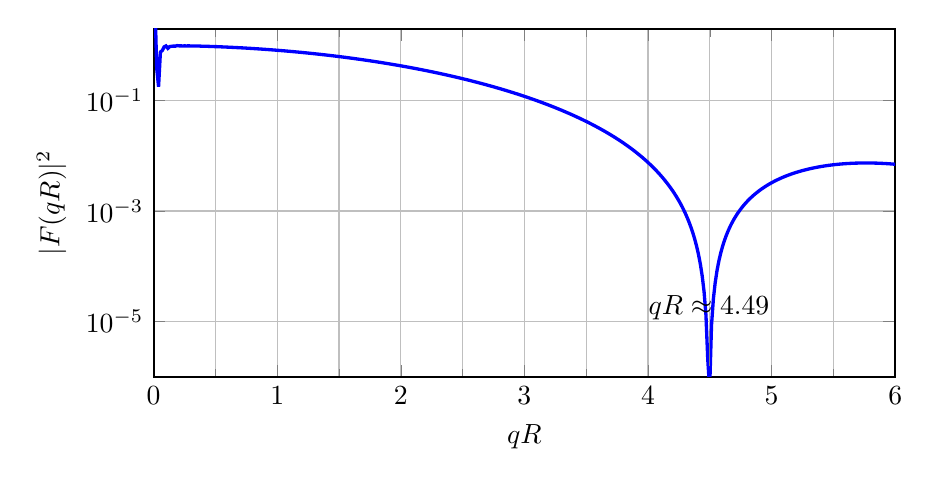
\begin{tikzpicture}
\begin{axis}[
  width=11cm, height=6cm,
  xlabel={$qR$}, ylabel={$|F(qR)|^{2}$},
  ymode=log, ymin=1e-6, ymax=2,
  xmin=0, xmax=6,
  domain=0.01:6, samples=400,
  grid=both, minor tick num=1,
  thick
]
\addplot[blue, very thick] {(3*(sin(deg(x)) - x*cos(deg(x)))/(x^3))^2};
\node at (axis cs:4.493,1e-6) [pin=above:{$qR\approx 4.49$}] {};
\end{axis}
\end{tikzpicture}
\end{center}

\subsection*{(b) Limits $q\to 0$, $q\to\infty$, and softening of minima}

Taylor-expand sine and cosine to order $x^{5}$:
\[
\sin x-x\cos x\;=\;\bigl(x-\tfrac{x^{3}}{6}+\tfrac{x^{5}}{120}\bigr)-\bigl(x-\tfrac{x^{3}}{2}+\tfrac{x^{5}}{24}\bigr).
\]
Combine like powers:
\[
\sin x-x\cos x\;=\;\tfrac{x^{3}}{3}-\tfrac{x^{5}}{30}+\dots
\]
Multiply by $3/x^{3}$ with $x=qR$:
\[
F(q)\;=\;1-\tfrac{1}{10}(qR)^{2}+\dots\;=\;1-\tfrac{1}{6}q^{2}\langle r^{2}\rangle+\dots
\]
Read off $\langle r^{2}\rangle=\tfrac{3}{5}R^{2}$. Hence
\begin{equation}
\boxed{\;\lim_{q\to 0}F(q)\;=\;1\;.}
\label{eq:F-q0}
\end{equation}
Charge conservation: a long-wavelength probe sees only $Ze$.

Large-$qR$: the bracket in \eqref{eq:F-uniform} is bounded while $(qR)^{3}\to\infty$:
\begin{equation}
\boxed{\;\lim_{q\to\infty}F(q)\;=\;0\;.}
\label{eq:F-qinf}
\end{equation}
Short-wavelength contributions interfere destructively over the volume.

\emph{Softening of the minima.} The exact zero is an artefact of the hard edge. Filling-in mechanisms: (i) Woods--Saxon surface diffuseness $a\sim\SI{0.5}{fm}$; (ii) intrinsic proton form factor $F_{p}(q)$ multiplying $F(q)$; (iii) Coulomb distortion / two-photon exchange (beyond first Born); (iv) inelastic excitation and recoil. Surface diffuseness is the dominant effect.

\subsection*{(c) Relativistic correction to Rutherford scattering}

Rutherford assumes non-relativistic spinless point charges in a Coulomb field. For $E\gtrsim m_{e}c^{2}$ two effects enter.

Apply $E^{2}=p^{2}c^{2}+m_{e}^{2}c^{4}$:
\[
E\;\neq\;p^{2}/2m_{e}\quad\text{(relativistic kinematics)}.
\]
Include Dirac spin coupling to the magnetic field in the nuclear rest frame (Mott):
\begin{equation}
\left(\frac{\de\sigma}{\de\Omega}\right)_\text{Mott}\;=\;\left(\frac{\de\sigma}{\de\Omega}\right)_\text{Ruth}\bigl[1-\beta^{2}\sin^{2}(\theta/2)\bigr].
\label{eq:Mott}
\end{equation}
Backward suppression as $\beta\to 1$: helicity conservation forbids the $180^{\circ}$ flip in the $m_{e}\to 0$ limit. (Nuclear recoil and $|F(q)|^{2}$ further required.)

\subsection*{(d) Determining $\rho(r)$ and the minimum energy to resolve $R=\SI{3}{fm}$}

\emph{Procedure.} Measure $\de\sigma/\de\Omega(\theta)$ at fixed $E_{\rm beam}$; divide by Mott (with recoil) to extract $|F(q)|^{2}$; fit $\rho(r;\{\alpha_{i}\})$ (Fermi / sum-of-Gaussians) so that \eqref{eq:F-spherical} reproduces the data; inverse Fourier transform yields $\rho(r)$.

To resolve the first diffraction minimum:
\[
qR\;\gtrsim\;4.49.
\]
Solve for $q$ at $R=\SI{3}{fm}$ using $\hbar c=\SI{197}{MeV.fm}$:
\[
qc\;\gtrsim\;\frac{4.49\times \SI{197}{MeV.fm}}{\SI{3}{fm}}.
\]
Evaluate:
\[
qc\;\gtrsim\;\SI{295}{MeV}.
\]
Ultra-relativistic backscattering ($\theta=\pi$): $q_{\max}\simeq 2p\approx 2E/c$:
\[
E_{\min}\;\simeq\;\tfrac{1}{2}q_{\max}c.
\]
Substitute $q_{\max}c=\SI{295}{MeV}$:
\[
E_{\min}\;\simeq\;\tfrac{1}{2}\times\SI{295}{MeV}.
\]
\begin{equation}
\boxed{\;E_{\min}\;\approx\;\SI{150}{MeV}\;.}
\label{eq:Emin}
\end{equation}
Weaker criterion $qR\sim\pi$ gives $E_{\min}\approx\SI{100}{MeV}$.

% =========================================================================
\section*{Question 2 --- Semi-Empirical Mass Formula and the nuclear force}

\textbf{Problem.} Origin of the $A$ and $A^{2/3}$ terms; uncertainty estimate of $p^{2}$; size of a $100\times$-Coulomb two-nucleon bound state. Exchange-force mass; $pn$ peaks. Stable $Z$ on the odd-$A$ parabola; pairing and even-$A$ stability.

\subsection*{(a) Saturation of the nuclear force, the volume and surface terms}

Empirical: $r=r_{0}A^{1/3}$ with $r_{0}\approx\SI{1.2}{fm}$, so $V\propto A$ and central density is constant (saturation); $BE/A\sim\SI{8}{MeV}$. Both demand short-range $NN$ force with hard core. Long-range force would give $BE\propto A(A-1)/2\propto A^{2}$, contradicting saturation.

Volume term $a_{V}A$: each interior nucleon has the same number of nearest neighbours.
Surface term $-a_{S}A^{2/3}$: surface nucleons lack neighbours, count $\propto 4\pi R^{2}\propto A^{2/3}$, sign negative.

\paragraph{Uncertainty-principle estimate of $p^{2}$.} Confinement $\Delta x\sim r$:
\begin{equation}
p^{2}\;\sim\;(\Delta p)^{2}\;\sim\;\frac{\hbar^{2}}{r^{2}}.
\label{eq:HUP}
\end{equation}
Kinetic energy $T=p^{2}/2m_{N}\sim\hbar^{2}/(2m_{N}r^{2})$ rises as $r\to 0$, opposing attraction.

\paragraph{Two-nucleon bound state with $V=-100\,e^{2}/(4\pi\epsilon_{0}r)$.} Effective coupling $\alpha_\text{eff}=100\alpha=100/137\approx 0.73$; reduced mass $\mu=m_{N}/2$.

Variational energy with $T=p^{2}/(2\mu)=\hbar^{2}/(2\mu r^{2})$:
\[
E(r)\;=\;\frac{\hbar^{2}}{2\mu r^{2}}-\frac{100\alpha\,\hbar c}{r}.
\]
Differentiate and set $\de E/\de r=0$:
\[
-\frac{\hbar^{2}}{\mu r^{3}}+\frac{100\alpha\,\hbar c}{r^{2}}\;=\;0.
\]
Multiply by $r^{3}$ and rearrange:
\[
100\alpha\,\hbar c\,r\;=\;\frac{\hbar^{2}}{\mu}.
\]
Solve for $r$:
\[
r_{\min}\;=\;\frac{\hbar^{2}}{\mu\,(100\alpha)\,\hbar c}\;=\;\frac{\hbar c}{(\mu c^{2})\,(100\alpha)}.
\]
Substitute $\mu c^{2}=m_{N}c^{2}/2\approx\SI{469.5}{MeV}$, $\hbar c=\SI{197}{MeV.fm}$, $100\alpha\approx 0.73$:
\[
r_{\min}\;=\;\frac{\SI{197}{MeV.fm}}{\SI{469.5}{MeV}\times 0.73}.
\]
Evaluate the denominator:
\[
r_{\min}\;=\;\frac{197}{342.7}\,\text{fm}.
\]
\begin{equation}
\boxed{\;r_{\min}\;\approx\;\SI{0.6}{fm}\;.}
\label{eq:rmin-final}
\end{equation}
Order of the deuteron radius ($\sim\SI{2}{fm}$): a $100\times$-Coulomb model captures the strong-force scale to a factor of a few.

\subsection*{(b) Exchange forces, Yukawa range, and the $pn$ scattering peaks}

Virtual exchange of mass $m_{X}$, lifetime $\Delta t\sim\hbar/(m_{X}c^{2})$, range $r\lesssim c\,\Delta t$:
\begin{equation}
R_\text{Yuk}\;=\;\frac{\hbar}{m_{X}c}.
\label{eq:Yukawa-range}
\end{equation}
Identify with $r_{0}=\SI{1.2}{fm}$:
\[
m_{X}c^{2}\;\sim\;\frac{\hbar c}{r_{0}}\;=\;\frac{\SI{197}{MeV.fm}}{\SI{1.2}{fm}}.
\]
\begin{equation}
\boxed{\;m_{X}c^{2}\;\approx\;\SI{160}{MeV}\;.}
\label{eq:mX}
\end{equation}
Compare $m_{\pi}\approx\SI{140}{MeV/c^{2}}$ (Yukawa).

\paragraph{Forward and backward peaks in $pn$ scattering.} Charge-exchange $\pi^{\pm}$ swaps proton and neutron identities:
\[
p+n\;\to\;n+p\quad(\pi^{\pm}\text{ exchange}).
\]
A forward neutron in the lab corresponds to a ``backward proton'' in the original-proton frame, producing a peak at $\theta_{p}=180^{\circ}$. The backward peak is direct evidence of the exchange-force component of the $NN$ interaction.

\subsection*{(c) Mass parabola, $\beta$-decay channels, and the role of pairing}

For fixed $A$, $BE$ is quadratic in $Z$:
\begin{equation}
BE(Z,A)\;=\;\text{($Z$-indep.)}-a_{C}\frac{Z^{2}}{A^{1/3}}-a_{A}\frac{(Z-A/2)^{2}}{A}\pm\delta(A,Z).
\label{eq:semf-Zfix}
\end{equation}
Atomic mass $M(Z,A)=Zm_{p}+(A-Z)m_{n}-BE/c^{2}$ is also quadratic in $Z$. For odd-$Z$ even-$N$ ($o\!-\!e$) isobars $\delta=0$, so all such isobars lie on a single parabola.

Stationary point of $M(Z,A)c^{2}=Zm_{p}c^{2}+(A-Z)m_{n}c^{2}-BE$:
\[
\pd{(Mc^{2})}{Z}\;=\;(m_{p}-m_{n})c^{2}-\pd{BE}{Z}\;=\;0.
\]
Compute $\partial BE/\partial Z$ from \eqref{eq:semf-Zfix}:
\[
\pd{BE}{Z}\;=\;-\frac{2a_{C}Z}{A^{1/3}}+a_{A}\frac{A-2Z}{A}.
\]
Substitute and rearrange:
\[
-\frac{2a_{C}Z}{A^{1/3}}+a_{A}\frac{A-2Z}{A}+(m_{n}-m_{p})c^{2}\;=\;0.
\]
Drop the small $(m_{n}-m_{p})c^{2}\!\ll\!a_{A}$ term:
\[
-\frac{2a_{C}Z}{A^{1/3}}+a_{A}-\frac{2a_{A}Z}{A}\;=\;0.
\]
Collect $Z$ on one side:
\[
a_{A}\;=\;2Z\!\left(\frac{a_{C}}{A^{1/3}}+\frac{a_{A}}{A}\right).
\]
Multiply numerator and denominator inside by $A$:
\[
a_{A}\;=\;\frac{2Z\,(a_{C}A^{2/3}+a_{A})}{A}.
\]
Solve for $Z$:
\begin{equation}
\boxed{\;Z_{\min}(A)\;\approx\;\frac{A/2}{1+(a_{C}/a_{A})\,A^{2/3}}\;.}
\label{eq:Zstab}
\end{equation}
Using $a_{C}\approx\SI{0.71}{MeV}$, $a_{A}\approx\SI{23}{MeV}$: light $A\Rightarrow Z_{\min}\approx A/2$ (i.e.\ $N=Z$); heavy $A\sim 200\Rightarrow Z_{\min}/A\approx 0.4$.

\paragraph{Three decay channels for unstable isobars.}
\begin{enumerate}
\item $\beta^{-}$: $n\to p+e^{-}+\bar\nu_{e}$ ($Z<Z_{\min}$, $\Delta Z=+1$).
\item $\beta^{+}$: $p\to n+e^{+}+\nu_{e}$ ($Z>Z_{\min}$, $Q>2m_{e}c^{2}\approx\SI{1.022}{MeV}$, $\Delta Z=-1$).
\item Electron capture: $p+e^{-}_\text{atomic}\to n+\nu_{e}$ ($Q>0$, $\Delta Z=-1$); dominates $\beta^{+}$ in heavy nuclei (no $2m_{e}c^{2}$ phase-space penalty, large inner-shell overlap).
\end{enumerate}

\paragraph{Pairing for $e\!-\!e$ and $o\!-\!o$ isobars.} Empirically
\begin{equation}
\delta\;\approx\;\begin{cases}+a_{P}/A^{1/2},& e\!-\!e\text{ (more bound)},\\ 0,& o\!-\!e,\\ -a_{P}/A^{1/2},& o\!-\!o\text{ (less bound)},\end{cases}
\label{eq:pairing}
\end{equation}
$a_{P}\approx\SI{12}{MeV}$. For even $A$, $e\!-\!e$ and $o\!-\!o$ chains lie on \emph{two} parabolae offset by $\sim 2a_{P}/A^{1/2}$.

Consequence: an $e\!-\!e$ isobar can be stable even off the parabola minimum, because the only single-$\beta$ neighbour is the less-bound $o\!-\!o$ isobar one step away. Example $A=128$: $^{128}$Te and $^{128}$Xe ($e\!-\!e$) both stable, separated by $^{128}$I ($o\!-\!o$) above; only $2\beta$-decay $^{128}\text{Te}\to{}^{128}\text{Xe}+2e^{-}+2\bar\nu_{e}$ connects them, $\tau\sim 10^{24}\,$yr. Empirical census: $\sim 165$ stable $e\!-\!e$ nuclei, only 4 stable $o\!-\!o$ ($^{2}$H, $^{6}$Li, $^{10}$B, $^{14}$N).

% =========================================================================
\section*{Question 3 --- The pseudoscalar meson nonet}

\textbf{Problem.} Identify the axes of the $J^{P}=0^{-}$ nonet; derive $J^{P}$ and $Q=I_{3}+S/2$ from quark content; show single-body decay forbidden; draw $\pi^{0}\to\gamma\gamma$; estimate Dalitz suppressions; explain BR$(\eta\to\gamma\gamma)<$BR$(\pi^{0}\to\gamma\gamma)$. Charged $\pi,K$ decay via virtual $W$; long lifetime; why $K^{0}$ cannot mimic $\pi^{0}$.

\subsection*{(a) Axes of the multiplet}

Horizontal: $I_{3}$. Vertical: $S$. Quark assignments: $u\,(I_{3}{=}{+}1/2,S{=}0)$, $d\,(I_{3}{=}{-}1/2,S{=}0)$, $s\,(I_{3}{=}0,S{=}{-}1)$; antiquarks flip sign. The $I_{3}$--$S$ plane is one face of the SU(3)$_\text{flav}$ weight diagram.

\subsection*{(b) Spin, parity, charge formula and the nonet}

Quarks are spin-$1/2$ fermions; for $L=0$:
\[
J\;=\;S_\text{tot}\;\in\;\{0,1\}.
\]
Intrinsic parity of $q\bar q$:
\[
P\;=\;P_{q}P_{\bar q}(-1)^{L}\;=\;(+1)(-1)(+1)\;=\;-1.
\]
Hence
\begin{equation}
J^{P}_\text{nonet}\;=\;0^{-}\quad(S_\text{tot}=0,\,L=0).
\label{eq:JP}
\end{equation}

\paragraph{Gell-Mann--Nishijima.} Quark charges: $Q_{u}=+2/3,Q_{d}=Q_{s}=-1/3$. With $B_{q}=1/3$:
\[
Q\;=\;I_{3}+\tfrac{1}{2}(S+B).
\]
For a meson $B=B_{q}+B_{\bar q}=0$:
\begin{equation}
\boxed{\;Q_\text{meson}\;=\;I_{3}+\frac{S}{2}\;.}
\label{eq:Q-meson}
\end{equation}
Check $K^{+}(I_{3}={+}1/2,S={+}1)$: $Q=1$. Check $\pi^{+}(I_{3}={+}1,S=0)$: $Q=1$. Check $\bar K^{0}(I_{3}={+}1/2,S={-}1)$: $Q=0$.

\paragraph{Why nine mesons.} Three flavours: $3\otimes\bar 3=8\oplus 1$. Octet $(\pi^{\pm,0},K^{\pm,0,\bar 0},\eta_{8})$ plus singlet $\eta_{1}$; physical $\eta,\eta'$ mix.

\paragraph{Why none stable.} Each has an open channel. $\pi^{0},\eta,\eta'$: electromagnetic $\to\gamma\gamma$. Charged $\pi,K$ and $K^{0}$: weak (virtual $W$). $\eta'$: strong $\eta'\to\eta\pi\pi$. No absolutely conserved quantum number forbids the lightest open channel.

\subsection*{(c) Single-body decay forbidden, $\pi^{0}\to\gamma\gamma$ and Dalitz suppressions}

Parent $M$ at rest, single daughter $m$. Energy conservation: $E_{f}=Mc^{2}$. Momentum conservation: $\vb p_{f}=0$.
Apply $E_{f}^{2}=p_{f}^{2}c^{2}+m^{2}c^{4}$:
\[
E_{f}^{2}\;=\;m^{2}c^{4}.
\]
Take the positive root and equate to $Mc^{2}$:
\[
Mc^{2}\;=\;mc^{2}.
\]
Hence $M=m$, impossible for a genuine decay; require $\geq 2$ daughters. Lightest pair for $\pi^{0}$: $\gamma\gamma$.

\paragraph{Feynman diagram for $\pi^{0}\to\gamma\gamma$.}
\begin{center}
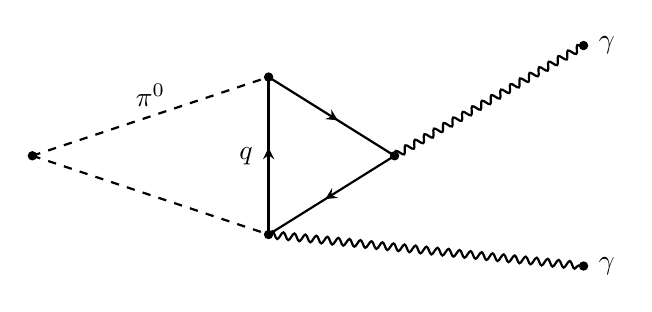
\begin{tikzpicture}[
  >=stealth,
  qline/.style={draw, thick, postaction={decorate,decoration={markings,mark=at position 0.55 with {\arrow{>}}}}},
  ph/.style={decorate, decoration={snake, amplitude=1.3pt, segment length=4pt}, draw, thick}
  ]
  \coordinate (P) at (-3,0);
  \coordinate (A) at (0,1);
  \coordinate (B) at (1.6,0);
  \coordinate (C) at (0,-1);
  \coordinate (G1) at (4,1.4);
  \coordinate (G2) at (4,-1.4);

  \draw[dashed, thick] (P) -- node[midway, above]{$\pi^{0}$} (A);
  \draw[dashed, thick] (P) -- (C);
  \fill (P) circle (1.7pt);
  \fill (A) circle (1.7pt);
  \fill (B) circle (1.7pt);
  \fill (C) circle (1.7pt);
  \fill (G1) circle (1.7pt);
  \fill (G2) circle (1.7pt);
  \draw[qline] (A) -- (B);
  \draw[qline] (B) -- (C);
  \draw[qline] (C) -- (A) node[midway, left=2pt]{$q$};
  \draw[ph] (B) -- (G1);
  \draw[ph] (C) -- (G2);
  \node[right=2pt] at (G1) {$\gamma$};
  \node[right=2pt] at (G2) {$\gamma$};
\end{tikzpicture}
\end{center}

\paragraph{Suppression of Dalitz channels.} Each replaced photon $\to e^{+}e^{-}$ adds one $\gamma e^{+}e^{-}$ vertex, i.e.\ one factor of $\alpha$ in the rate.

Single Dalitz:
\begin{equation}
\frac{\Gamma(\pi^{0}\to\gamma e^{+}e^{-})}{\Gamma(\pi^{0}\to\gamma\gamma)}\;\sim\;\alpha\;\approx\;\frac{1}{137}.
\label{eq:Dalitz1}
\end{equation}
Double Dalitz:
\begin{equation}
\frac{\Gamma(\pi^{0}\to e^{+}e^{-}e^{+}e^{-})}{\Gamma(\pi^{0}\to\gamma\gamma)}\;\sim\;\alpha^{2}\;\approx\;\frac{1}{1.9\times 10^{4}}.
\label{eq:Dalitz2}
\end{equation}
Measured: BR$(\pi^{0}\to\gamma e^{+}e^{-})=1.17\%$, BR$(\pi^{0}\to e^{+}e^{-}e^{+}e^{-})=3.3\times 10^{-5}$.

\paragraph{Why BR$(\eta\to\gamma\gamma)<$BR$(\pi^{0}\to\gamma\gamma)$.} The $\eta$ is heavier ($m_{\eta}\approx\SI{548}{MeV}$) so additional channels open ($3\pi^{0}$, $\pi^{+}\pi^{-}\pi^{0}$, $\pi^{+}\pi^{-}\gamma$,\dots) which are closed for the lighter $\pi^{0}$ ($m_{\pi^{0}}\approx\SI{135}{MeV}$). The extra phase space inflates the total width $\Gamma_{\eta}\approx\SI{1.3}{keV}\gg\Gamma_{\pi^{0}}\approx\SI{8}{eV}$ much more than the $\gamma\gamma$ partial width grows, so BR$(\gamma\gamma)$ falls:
\begin{equation}
\text{BR}(\eta\to\gamma\gamma)\;\approx\;39\%\;<\;\text{BR}(\pi^{0}\to\gamma\gamma)\;\approx\;99\%.
\label{eq:eta-vs-pi0}
\end{equation}

\subsection*{(d) Charged pion and kaon decays; the $K^{0}$ case}

$\pi^{+}=u\bar d$ annihilates into virtual $W^{+}\to\ell^{+}\nu_{\ell}$:
\begin{center}
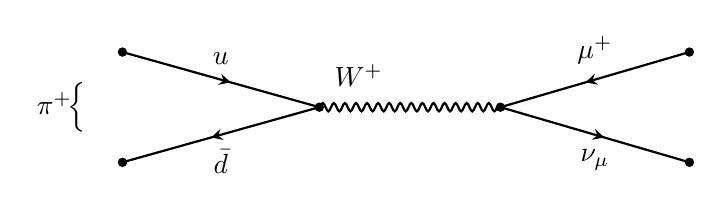
\begin{tikzpicture}[
  >=stealth,
  qline/.style={draw, thick, postaction={decorate,decoration={markings,mark=at position 0.55 with {\arrow{>}}}}},
  W/.style={decorate, decoration={snake, amplitude=1.5pt, segment length=4pt}, draw, thick}
  ]
  \coordinate (u) at (-3,0.7);
  \coordinate (d) at (-3,-0.7);
  \coordinate (V) at (-0.5,0);
  \coordinate (W2) at (1.8,0);
  \coordinate (mu) at (4.2,0.7);
  \coordinate (nu) at (4.2,-0.7);
  \fill (u) circle (1.7pt);
  \fill (d) circle (1.7pt);
  \fill (V) circle (1.7pt);
  \fill (W2) circle (1.7pt);
  \fill (mu) circle (1.7pt);
  \fill (nu) circle (1.7pt);
  \draw[qline] (u) -- (V);
  \node[above=2pt] at ($(u)!0.5!(V)$) {$u$};
  \draw[qline] (V) -- (d);
  \node[below=2pt] at ($(V)!0.5!(d)$) {$\bar d$};
  \draw[W] (V) -- (W2);
  \node[midway, above=4pt] at ($(V)!0.5!(W2)$) {$W^{+}$};
  \draw[qline] (mu) -- (W2);
  \node[above=2pt] at ($(W2)!0.5!(mu)$) {$\mu^{+}$};
  \draw[qline] (W2) -- (nu);
  \node[below=2pt] at ($(W2)!0.5!(nu)$) {$\nu_{\mu}$};
  \node[left=4pt] at (-3.2,0) {$\pi^{+}\!\Big\{$};
\end{tikzpicture}
\end{center}

\paragraph{Why a heavy $W$ mediates a light decay.} The $W$ is virtual; energy-time uncertainty allows $\Delta t\sim\hbar/m_{W}c^{2}$; propagator $\sim 1/(q^{2}-m_{W}^{2}c^{2})\approx -1/(m_{W}c)^{2}$ at $q^{2}\ll m_{W}^{2}c^{2}$.

\paragraph{Why the lifetime is long.} Two factors.

Suppression by Fermi constant:
\[
\frac{G_{F}}{\sqrt{2}}\;=\;\frac{g_{w}^{2}}{8 m_{W}^{2}c^{4}}\quad(\text{small in natural units}).
\]
Helicity suppression in $\pi^{+}\to\ell^{+}\nu_{\ell}$ (spin-0 parent, $V{-}A$ couplings forces same-helicity $\ell^{+}\nu_{\ell}$ that is forbidden by back-to-back angular momentum unless $m_{\ell}\neq 0$):
\[
\Gamma\;\propto\;m_{\ell}^{2}(m_{\pi}^{2}-m_{\ell}^{2})^{2}.
\]
Together $\tau_{\pi^{\pm}}\approx\SI{2.6e-8}{s}$; eight orders of magnitude longer than strong decays and than $\tau_{\pi^{0}}\approx\SI{8e-17}{s}$.

\paragraph{Why $K^{0}$ cannot use the $\pi^{0}$ mode.} $K^{0}=d\bar s$, $S=+1$. Photon annihilation requires $q$ and $\bar q$ of the \emph{same} flavour, which $d\bar s$ is not; electromagnetism conserves flavour, so cannot turn $s\leftrightarrow d$. Only the weak interaction can change strangeness ($\Delta S=1$). Representative semileptonic ($K_{\ell 3}$) diagram for $K^{0}\to\pi^{-}\ell^{+}\nu_{\ell}$:
\begin{center}
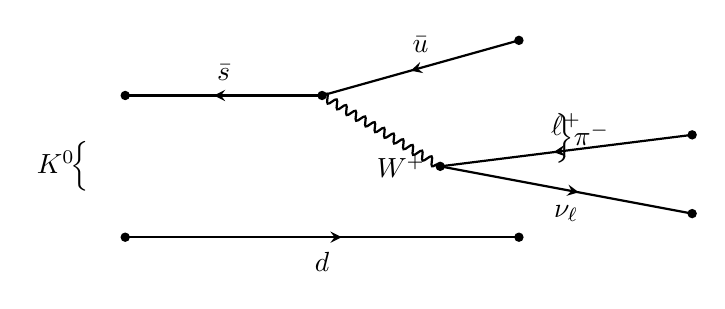
\begin{tikzpicture}[
  >=stealth,
  qline/.style={draw, thick, postaction={decorate,decoration={markings,mark=at position 0.55 with {\arrow{>}}}}},
  W/.style={decorate, decoration={snake, amplitude=1.5pt, segment length=4pt}, draw, thick}
  ]
  \coordinate (s)  at (-3.0, 0.9);
  \coordinate (d1) at (-3.0,-0.9);
  \coordinate (V)  at (-0.5, 0.9);
  \coordinate (u)  at ( 2.0, 1.6);
  \coordinate (d2) at ( 2.0,-0.9);
  \coordinate (W2) at ( 1.0, 0.0);
  \coordinate (lep)at ( 4.2, 0.4);
  \coordinate (nu) at ( 4.2,-0.6);
  \fill (s) circle (1.7pt);
  \fill (d1) circle (1.7pt);
  \fill (V) circle (1.7pt);
  \fill (u) circle (1.7pt);
  \fill (d2) circle (1.7pt);
  \fill (W2) circle (1.7pt);
  \fill (lep) circle (1.7pt);
  \fill (nu) circle (1.7pt);
  \draw[qline] (V) -- (s);
  \node[above=2pt] at ($(s)!0.5!(V)$) {$\bar s$};
  \draw[qline] (u) -- (V);
  \node[above=2pt] at ($(V)!0.5!(u)$) {$\bar u$};
  \draw[qline] (d1) -- (d2);
  \node[below=2pt] at ($(d1)!0.5!(d2)$) {$d$};
  \draw[W] (V) -- (W2);
  \node[midway, right=2pt] at ($(V)!0.5!(W2)$) {$W^{+}$};
  \draw[qline] (lep) -- (W2);
  \node[above=2pt] at ($(W2)!0.5!(lep)$) {$\ell^{+}$};
  \draw[qline] (W2) -- (nu);
  \node[below=2pt] at ($(W2)!0.5!(nu)$) {$\nu_{\ell}$};
  \node[left=4pt] at (-3.2,0) {$K^{0}\!\Big\{$};
  \node[right=4pt] at (2.2,0.35) {$\Big\}\pi^{-}$};
\end{tikzpicture}
\end{center}

% =========================================================================
\section*{Question 4 --- Lepton universality and quark mixing}

\textbf{Problem.} Diagrams for $\mu$ and $\tau$ decay; hadronic decays; justify $\Gamma(\tau\to e\nu\bar\nu)/\Gamma(\mu\to e\nu\bar\nu)\simeq(m_{\tau}/m_{\mu})^{5}(g_{\tau}/g_{\mu})^{2}$. Evaluate $g_{\tau}/g_{\mu}$. Quark-level diagrams for $n,\Lambda^{0}$ $\beta$-decay; restoration of universality via Cabibbo mixing; minimum quark count; $\theta_{C}$. Predict $\tau$ branching ratios; comment on heavy-quark stability.

\subsection*{(a) Leptonic decays and the $m^{5}$ scaling}

\paragraph{Feynman diagrams.}
\begin{center}
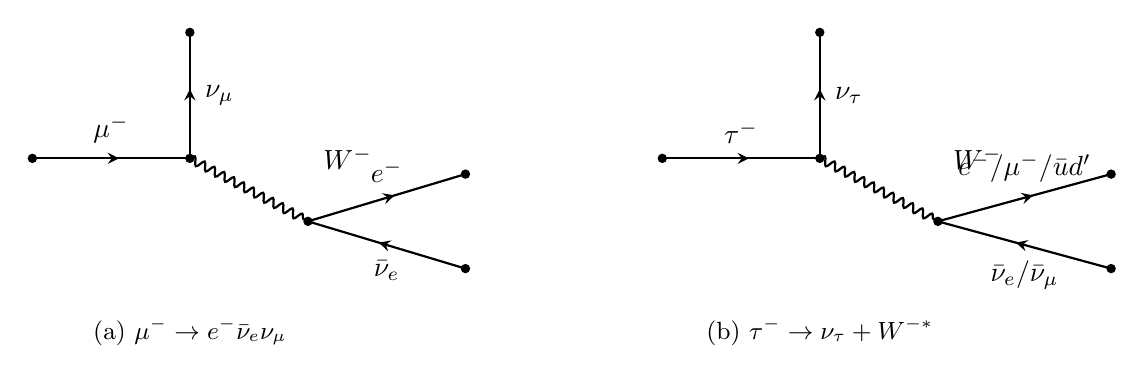
\begin{tikzpicture}[
  >=stealth,
  qline/.style={draw, thick, postaction={decorate,decoration={markings,mark=at position 0.55 with {\arrow{>}}}}},
  W/.style={decorate, decoration={snake, amplitude=1.5pt, segment length=4pt}, draw, thick}
  ]
  % muon decay
  \coordinate (mu)  at (-3.5, 0);
  \coordinate (V1)  at (-1.5, 0);
  \coordinate (numu) at (-1.5, 1.6);
  \coordinate (W1)  at ( 0.0,-0.8);
  \coordinate (e1)  at ( 2.0,-0.2);
  \coordinate (nue1) at ( 2.0,-1.4);
  \fill (mu) circle (1.7pt);
  \fill (V1) circle (1.7pt);
  \fill (numu) circle (1.7pt);
  \fill (W1) circle (1.7pt);
  \fill (e1) circle (1.7pt);
  \fill (nue1) circle (1.7pt);
  \draw[qline] (mu) -- (V1);
  \node[above=2pt] at ($(mu)!0.5!(V1)$) {$\mu^{-}$};
  \draw[qline] (V1) -- (numu);
  \node[right=2pt] at ($(V1)!0.5!(numu)$) {$\nu_{\mu}$};
  \draw[W] (V1) -- (W1);
  \node[midway, right=2pt] at ($(V1)!0.5!(W1)$) {$W^{-}$};
  \draw[qline] (W1) -- (e1);
  \node[above=2pt] at ($(W1)!0.5!(e1)$) {$e^{-}$};
  \draw[qline] (nue1) -- (W1);
  \node[below=2pt] at ($(W1)!0.5!(nue1)$) {$\bar\nu_{e}$};
  \node[font=\small] at (-1.5,-2.2) {(a) $\mu^{-}\to e^{-}\bar\nu_{e}\nu_{\mu}$};

  \begin{scope}[xshift=8cm]
  \coordinate (mu)  at (-3.5, 0);
  \coordinate (V1)  at (-1.5, 0);
  \coordinate (numu) at (-1.5, 1.6);
  \coordinate (W1)  at ( 0.0,-0.8);
  \coordinate (e1)  at ( 2.2,-0.2);
  \coordinate (nue1) at ( 2.2,-1.4);
  \fill (mu) circle (1.7pt);
  \fill (V1) circle (1.7pt);
  \fill (numu) circle (1.7pt);
  \fill (W1) circle (1.7pt);
  \fill (e1) circle (1.7pt);
  \fill (nue1) circle (1.7pt);
  \draw[qline] (mu) -- (V1);
  \node[above=2pt] at ($(mu)!0.5!(V1)$) {$\tau^{-}$};
  \draw[qline] (V1) -- (numu);
  \node[right=2pt] at ($(V1)!0.5!(numu)$) {$\nu_{\tau}$};
  \draw[W] (V1) -- (W1);
  \node[midway, right=2pt] at ($(V1)!0.5!(W1)$) {$W^{-}$};
  \draw[qline] (W1) -- (e1);
  \node[above=2pt] at ($(W1)!0.5!(e1)$) {$e^{-}/\mu^{-}/\bar u d'$};
  \draw[qline] (nue1) -- (W1);
  \node[below=2pt] at ($(W1)!0.5!(nue1)$) {$\bar\nu_{e}/\bar\nu_{\mu}$};
  \node[font=\small] at (-1.5,-2.2) {(b) $\tau^{-}\to\nu_{\tau}+W^{-*}$};
  \end{scope}
\end{tikzpicture}
\end{center}

\emph{Hadronic decays.} $m_{\mu}c^{2}\approx\SI{106}{MeV}<m_{\pi}\approx\SI{140}{MeV}$: muon hadronic decay forbidden. $m_{\tau}c^{2}\approx\SI{1777}{MeV}\gg m_{\pi}$: $\tau\to\nu_{\tau}+\bar u d'$ allowed; charm channels closed since $m_{D}\approx\SI{1870}{MeV/c^{2}}>m_{\tau}c^{2}$; quarks hadronise.

\paragraph{The $m^{5}$ rule.} For $m_{\ell}\ll m_{W}$, the $W$ propagator contracts to a four-fermion contact:
\[
\mathcal{L}_\text{eff}\;\propto\;\frac{g_{\ell}g_{e}}{m_{W}^{2}}\,(\bar\nu_{\ell}\ell)(\bar e\nu_{e}).
\]
Three-body massless phase space scales as $m_{\ell}^{5}$ (only available scale, $G_{F}$ has dimension [E]$^{-2}$). Standard result:
\begin{equation}
\Gamma(\ell^{-}\to\nu_{\ell}e^{-}\bar\nu_{e})\;=\;\frac{g_{\ell}^{2}g_{e}^{2}}{192\pi^{3}}\,\frac{m_{\ell}^{5}c^{4}}{m_{W}^{4}\hbar}.
\label{eq:rate-leptonic}
\end{equation}
Form the ratio for $\tau$ over $\mu$ ($g_{e}$ cancels):
\begin{equation}
\boxed{\;\frac{\Gamma(\tau^{-}\to e^{-}\bar\nu_{e}\nu_{\tau})}{\Gamma(\mu^{-}\to e^{-}\bar\nu_{e}\nu_{\mu})}\;=\;\left(\frac{m_{\tau}}{m_{\mu}}\right)^{5}\!\left(\frac{g_{\tau}}{g_{\mu}}\right)^{2}\;.}
\label{eq:m5}
\end{equation}

\subsection*{(b) Numerical evaluation of $g_{\tau}/g_{\mu}$}

Widths from lifetimes:
\[
\Gamma(\tau\to e\nu\bar\nu)\;=\;\frac{\hbar\,\text{BR}(\tau\to e\nu\bar\nu)}{\tau_{\tau}},\qquad\Gamma(\mu)\;=\;\frac{\hbar}{\tau_{\mu}}\;(\text{BR}=1).
\]
Form the ratio:
\[
\frac{\Gamma_{\tau}^{(e)}}{\Gamma_{\mu}}\;=\;\frac{\tau_{\mu}}{\tau_{\tau}}\,\text{BR}(\tau\to e\nu\bar\nu).
\]
Substitute $\tau_{\mu}=2.197\times 10^{-6}\,$s, $\tau_{\tau}=2.91\times 10^{-13}\,$s, BR$=0.178$:
\[
\frac{\Gamma_{\tau}^{(e)}}{\Gamma_{\mu}}\;=\;\frac{2.197\times 10^{-6}}{2.91\times 10^{-13}}\times 0.178.
\]
Evaluate the lifetime ratio:
\[
\frac{\tau_{\mu}}{\tau_{\tau}}\;\approx\;7.55\times 10^{6}.
\]
Multiply by BR:
\[
\frac{\Gamma_{\tau}^{(e)}}{\Gamma_{\mu}}\;\approx\;7.55\times 10^{6}\times 0.178\;\approx\;1.344\times 10^{6}.
\]
Mass-ratio factor:
\[
\frac{m_{\tau}}{m_{\mu}}\;=\;\frac{1777.0}{105.66}\;\approx\;16.82.
\]
Raise to the fifth power:
\[
\left(\frac{m_{\tau}}{m_{\mu}}\right)^{5}\;=\;(16.82)^{5}\;\approx\;1.346\times 10^{6}.
\]
Take the ratio of \eqref{eq:m5}:
\[
\left(\frac{g_{\tau}}{g_{\mu}}\right)^{2}\;=\;\frac{1.344\times 10^{6}}{1.346\times 10^{6}}\;\approx\;0.998.
\]
\begin{equation}
\boxed{\;\frac{g_{\tau}}{g_{\mu}}\;\approx\;1.00\;.}
\label{eq:gtau-over-gmu}
\end{equation}
Lepton universality at the $W$ vertex.

\subsection*{(c) Quark-level Feynman diagrams for $n$ and $\Lambda^{0}$ decay}

\begin{center}
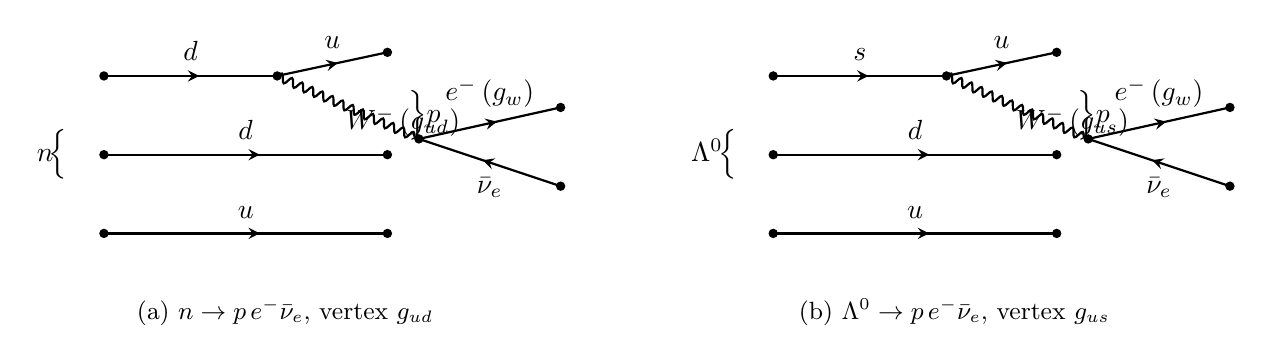
\begin{tikzpicture}[
  >=stealth,
  qline/.style={draw, thick, postaction={decorate,decoration={markings,mark=at position 0.55 with {\arrow{>}}}}},
  W/.style={decorate, decoration={snake, amplitude=1.5pt, segment length=4pt}, draw, thick}
  ]
  % Neutron
  \coordinate (d1) at (-3.8, 1.0);
  \coordinate (d2) at (-3.8, 0.0);
  \coordinate (u1) at (-3.8,-1.0);
  \coordinate (V)  at (-1.6, 1.0);
  \coordinate (uout) at (-0.2, 1.3);
  \coordinate (Wend) at ( 0.2, 0.2);
  \coordinate (e)   at ( 2.0, 0.6);
  \coordinate (nu)  at ( 2.0,-0.4);
  \fill (d1) circle (1.7pt);
  \fill (d2) circle (1.7pt);
  \fill (u1) circle (1.7pt);
  \fill (V) circle (1.7pt);
  \fill (uout) circle (1.7pt);
  \fill (Wend) circle (1.7pt);
  \fill (e) circle (1.7pt);
  \fill (nu) circle (1.7pt);
  \draw[qline] (d1) -- (V);
  \node[above=2pt] at ($(d1)!0.5!(V)$) {$d$};
  \draw[qline] (V) -- (uout);
  \node[above=2pt] at ($(V)!0.5!(uout)$) {$u$};
  \draw[qline] (d2) -- (-0.2,0.0);
  \fill (-0.2,0) circle (1.7pt);
  \node[above=2pt] at ($(d2)!0.5!(-0.2,0)$) {$d$};
  \draw[qline] (u1) -- (-0.2,-1.0);
  \fill (-0.2,-1) circle (1.7pt);
  \node[above=2pt] at ($(u1)!0.5!(-0.2,-1)$) {$u$};
  \draw[W] (V) -- (Wend);
  \node[midway, above=3pt] at ($(V)!0.5!(Wend)$) {$W^{-}\,(g_{ud})$};
  \draw[qline] (Wend) -- (e);
  \node[above=2pt] at ($(Wend)!0.5!(e)$) {$e^{-}\,(g_{w})$};
  \draw[qline] (nu) -- (Wend);
  \node[below=2pt] at ($(Wend)!0.5!(nu)$) {$\bar\nu_{e}$};
  \node[left=4pt] at (-4.0,0) {$n\!\Big\{$};
  \node[right=4pt] at (-0.2,0.5) {$\Big\}p$};
  \node[font=\small] at (-1.5,-2.0) {(a) $n\to p\,e^{-}\bar\nu_{e}$, vertex $g_{ud}$};

  \begin{scope}[xshift=8.5cm]
  \coordinate (s1) at (-3.8, 1.0);
  \coordinate (d2) at (-3.8, 0.0);
  \coordinate (u1) at (-3.8,-1.0);
  \coordinate (V)  at (-1.6, 1.0);
  \coordinate (uout) at (-0.2, 1.3);
  \coordinate (Wend) at ( 0.2, 0.2);
  \coordinate (e)   at ( 2.0, 0.6);
  \coordinate (nu)  at ( 2.0,-0.4);
  \fill (s1) circle (1.7pt);
  \fill (d2) circle (1.7pt);
  \fill (u1) circle (1.7pt);
  \fill (V) circle (1.7pt);
  \fill (uout) circle (1.7pt);
  \fill (Wend) circle (1.7pt);
  \fill (e) circle (1.7pt);
  \fill (nu) circle (1.7pt);
  \draw[qline] (s1) -- (V);
  \node[above=2pt] at ($(s1)!0.5!(V)$) {$s$};
  \draw[qline] (V) -- (uout);
  \node[above=2pt] at ($(V)!0.5!(uout)$) {$u$};
  \draw[qline] (d2) -- (-0.2,0.0);
  \fill (-0.2,0) circle (1.7pt);
  \node[above=2pt] at ($(d2)!0.5!(-0.2,0)$) {$d$};
  \draw[qline] (u1) -- (-0.2,-1.0);
  \fill (-0.2,-1) circle (1.7pt);
  \node[above=2pt] at ($(u1)!0.5!(-0.2,-1)$) {$u$};
  \draw[W] (V) -- (Wend);
  \node[midway, above=3pt] at ($(V)!0.5!(Wend)$) {$W^{-}\,(g_{us})$};
  \draw[qline] (Wend) -- (e);
  \node[above=2pt] at ($(Wend)!0.5!(e)$) {$e^{-}\,(g_{w})$};
  \draw[qline] (nu) -- (Wend);
  \node[below=2pt] at ($(Wend)!0.5!(nu)$) {$\bar\nu_{e}$};
  \node[left=4pt] at (-4.0,0) {$\Lambda^{0}\!\Big\{$};
  \node[right=4pt] at (-0.2,0.5) {$\Big\}p$};
  \node[font=\small] at (-1.5,-2.0) {(b) $\Lambda^{0}\to p\,e^{-}\bar\nu_{e}$, vertex $g_{us}$};
  \end{scope}
\end{tikzpicture}
\end{center}

In each diagram one quark of the parent emits a virtual $W^{-}$ and converts to a lighter quark; spectators rearrange.

\subsection*{(d) Universality restoration via Cabibbo mixing}

In the lepton sector $g_{w}$ is universal; for quarks $g_{ud}\neq g_{us}\neq g_{w}$. Cabibbo: weak-eigenstate $d'$ is a unitary rotation of mass eigenstates:
\begin{equation}
\begin{pmatrix}d'\\ s'\end{pmatrix}\;=\;\begin{pmatrix}\cos\theta_{C}&\sin\theta_{C}\\ -\sin\theta_{C}&\cos\theta_{C}\end{pmatrix}\begin{pmatrix}d\\ s\end{pmatrix}.
\label{eq:Cabibbo}
\end{equation}
Universal vertex in weak basis:
\[
g_{ud}\;=\;g_{w}\cos\theta_{C},\qquad g_{us}\;=\;g_{w}\sin\theta_{C}.
\]
Sum of squares:
\[
g_{ud}^{2}+g_{us}^{2}\;=\;g_{w}^{2}\quad(\text{universality restored}).
\]
\emph{Minimum quark count: four.} A $2\times 2$ rotation requires a partner up-type pair $(u,c)$, predicting charm (GIM, 1970; charm discovered 1974).

\paragraph{Determination of $\theta_{C}$.} From the data:
\[
\sin\theta_{C}\;=\;\frac{g_{us}}{g_{w}}\;\simeq\;0.221,\qquad\cos\theta_{C}\;=\;\frac{g_{ud}}{g_{w}}\;\simeq\;0.974.
\]
Solve:
\[
\theta_{C}\;\approx\;\arcsin(0.221).
\]
\begin{equation}
\boxed{\;\theta_{C}\;\approx\;12.8^{\circ}\;.}
\label{eq:thetaC-numbers}
\end{equation}
Unitarity check: $0.221^{2}+0.974^{2}=0.0488+0.949=0.998\approx 1$.

Strangeness-changing rate suppressed by $\tan^{2}\theta_{C}\approx 0.052$.

\subsection*{(e) Tau branching ratios from two-generation universality}

$W^{-}$ couples democratically to $e^{-}\bar\nu_{e},\mu^{-}\bar\nu_{\mu},\bar u d',\bar c s'$. Phase space $\sim m_{\tau}^{5}$ for each. Quark channels carry colour factor 3. Cabibbo unitarity: $\bar u d'\to\bar u d(\cos^{2}\theta_{C})+\bar u s(\sin^{2}\theta_{C})$, summing to one. Charm channels require a $D$ meson, $m_{D}\approx\SI{1865}{MeV/c^{2}}>m_{\tau}-m_{\nu}=\SI{1777}{MeV/c^{2}}$: kinematically forbidden.

Channel weights:
\begin{equation}
\begin{aligned}
\tau^{-}\to e^{-}\bar\nu_{e}\nu_{\tau}&:\quad 1,\\
\tau^{-}\to\mu^{-}\bar\nu_{\mu}\nu_{\tau}&:\quad 1,\\
\tau^{-}\to\nu_{\tau}+(\bar u d)&:\quad 3\cos^{2}\theta_{C}\approx 2.85,\\
\tau^{-}\to\nu_{\tau}+(\bar u s)&:\quad 3\sin^{2}\theta_{C}\approx 0.146,\\
\tau^{-}\to\nu_{\tau}+\bar c\dots&:\quad\text{forbidden}.
\end{aligned}
\label{eq:tau-channels}
\end{equation}
Total weight:
\[
W_\text{tot}\;=\;1+1+3(\cos^{2}\theta_{C}+\sin^{2}\theta_{C})\;=\;5.
\]
\begin{equation}
\boxed{\;\text{BR}(\tau^{-}\to e^{-}\bar\nu_{e}\nu_{\tau})\;=\;\tfrac{1}{5}\;=\;20\%\;.}
\label{eq:BR-e}
\end{equation}
\begin{equation}
\boxed{\;\text{BR}(\tau^{-}\to\mu^{-}\bar\nu_{\mu}\nu_{\tau})\;=\;\tfrac{1}{5}\;=\;20\%\;.}
\label{eq:BR-mu}
\end{equation}
\begin{equation}
\boxed{\;\text{BR}(\tau^{-}\to\nu_{\tau}+\text{hadrons})\;=\;\tfrac{3}{5}\;=\;60\%\;.}
\label{eq:BR-had}
\end{equation}
Measured: $17.8\%,17.4\%,\sim 65\%$; the deficit in the leptonic modes reflects QCD enhancement ($\sim\alpha_{s}/\pi$) of the hadronic width.

\paragraph{Consequences of mixing.} Mass and weak eigenstates differ, so $s,c,b,t$ are not weak eigenstates and must decay via $W$ to a lighter quark with strength set by CKM. Without mixing $s$ and $c$ would be stable; with mixing, all heavy quarks have non-zero decay widths and ordinary matter is dominated by the lightest generation $u,d$.

\end{document}
